\section{Auswahl DNS-Cloud-Serviceprovider}
Zunächst war es notwendig sich auf dem Markt umzusehen um geeignete Anbieter von Cloud-Dienstleistern zu identifizieren. Anschließend wurden Kriterien gewählt, anhand deren die Anzahl der Alternativen eingeschränkt wurde. 

Der Markt an DNS-Serviceprovidern ist enorm groß. Das meist genutzte Benchmark zum Vergleich von DNS-Services ist offensichtlich die benötigte Zeit zur direkten Auflösung einer DNS-Querry. Laut des DNS-Benchmarking Service \textit{DNSPerf} sind die Abweichungen der ersten 30 Plätze hier bei gerade einmal 30ms. Auch die Verfügbarkeit der einzelnen DNS-Server beläuft sich in den letzten 6 Monaten bei den ersten 30 Plätzen ebenfalls durchgängig bei 100\%. Bei anderen Benchmarking-Services waren ebenfalls ähnliche Werte zu verzeichnen. \cite{DNSPerf.2018}

Da eine Abweichung von 30ms bei der Bearbeitung einer DNS-Querry bei den meisten Endbenutzer im alltäglichen Gebrauch kaum ins Gewicht fallen dürfte, wurde dies im weiteren Verlauf nicht weiter berücksichtigt. Auch eine Verfügbarkeit von 100\% scheint dem allgemeinen Standard zu entsprechen.

Um trotzdem eine relevante und angemessene Auswahl eines DNS-Serviceproviders zu treffen, wurde der Fokus von DNS-Anbietern auf Anbieter von Cloud-Services allgemein verlagert. Von der Organisation RightScale wurde hierzu in diesem Jahr eine Umfrage mit über 1000 Beteiligten vorgenommen. Wie in Abbildung \ref{fig:cloudProvComp} zu sehen, wurden die größten Provider verglichen anhand gehosteter Applikationen. Es wurde ebenfalls unterteilt in Nutzer, die den Service derzeit nur Testen oder in Zukunft planen mit ihrer Anwendung zu dem Cloud-Dienstleister zu wechseln. Hierbei ist zu sehen, dass Amazon Web Service derzeit der Führende Anbieter von Cloud-Dienstleistungen darstellt. Auf dem zweiten Platz befindet sicher Microsoft mit ihrem Azure-Service, wobei hier ebenfalls das von Microsoft viel verkaufte Produkt \textit{Office-365} als \textit{Enterprise}-Lösung mit einbezogen wurde. \cite{ZDNet.2018b}

\begin{figure}[ht]
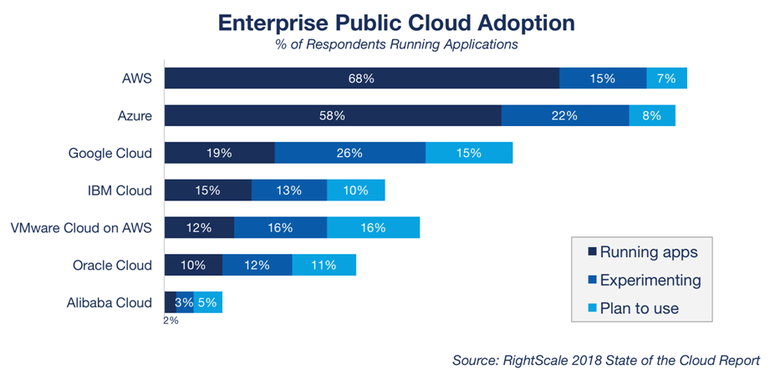
\includegraphics[width=\columnwidth]{images/rs_cloudComp.png}
\caption{Vergleich Cloud-Dienstleister auf der Basis gehosteter Applikationen}
\label{fig:cloudProvComp}
\end{figure}

Aufgrund der gezeigten Ergebnisse und der Benchmarks von \textit{DNSPref} wurden nun die Cloud-Anbieter festgelegt. Die zur Erstellung des Modells untersuchten DNS-Services lauten wie folgt:

\begin{tabular}{lll}
\raisebox{-.5\height}{
\includegraphics[width=55pt]{images/logo_aws.png}} & Amazon Web Services - Route 53 \\
\raisebox{-.5\height}{
\includegraphics[width=60pt]{images/logo_azure2.png}} & Microsoft Azure - DNS-Zonen \\ \\
\raisebox{-.5\height}{
\includegraphics[width=55pt]{images/logo_google.png}} & Google Cloud DNS\\ 
\\
\end{tabular}